% Chapter 5

\chapter{Calculation of radiative corrections} % Chapter title

\label{ch:Calculation} % For referencing the chapter elsewhere, use \autoref{ch:name}

%----------------------------------------------------------------------------------------

In the past, COMPASS has been using two programs for radiative corrections estimation : one is TERAD, a program that does analytic calculations of the ($x,y$)-dependant radiative correction factors, the other is RADGEN, which in addition to the ($x,y$)-dependant radiative correction factors allows one to take into account a kinematic smearing caused by the radiated photon. A third program is discussed within this thesis : DJANGOH. DJANGOH can compute radiative correction factors in bins of ($x,y,z$) and generate events with real photon emission.

\section{TERAD}

The TERAD program is based on calculations described in Refs \cite{TERAD1,TERAD2,TERAD3}. These calculations are also referred to as the Dubna radiative correction scheme. Both model-independent and QPM are used for computing the deep inelastic processes. An example of the former are radiative corrections to the leptonic current. The QPM is used for all other corrections, i.e. for computing the double photon exchange, real photon emission from quark lines, quark self-energy and weak loop corrections. Also implemented were the $O(\alpha^2)$ corrections, corresponding to $\alpha^4$ contributions to the cross-section. The diagrams corresponding to the $O(\alpha^2)$ corrections are shown in Fig.~\ref{pic:order2corr}.

\begin{figure}[!h]
  \centering
	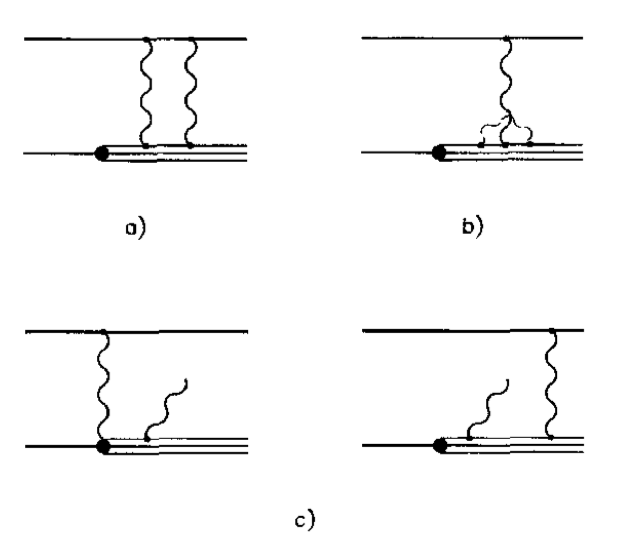
\includegraphics[scale=0.8]{./gfx/order2corr.png}
	\caption{$O(\alpha^2)$ corrections implemented inside TERAD. Double photon exchange (a) and hadron current corrections (b,c) in the Dubna scheme.}
	\label{pic:order2corr}
\end{figure}

%----------------------------------------------------------------------------------------

\section{RADGEN}

The RADGEN generator \cite{RADGEN} contains two patches which can be considered as independent generators. The first one is based on POLRAD$2.0$ \cite{POLRAD} and is used for polarized lepton-nucleon scattering. The second one is based on FERRAD$3.5$ \cite{FERRAD} and deals with the unpolarized case.
POLRAD$2.0$ is based on the method of covariant cancellation of infrared divergences developed by Bardin and Shumeiko \cite{BardinShu}. FERRAD$3.5$ is calculating the radiative corrections to DIS of unpolarized particles in accordance with the analytical fomulae given by Mo and Tsai \cite{MoTsai}. RADGEN is calculating the total radiative corrections at the lowest order. The Monte-Carlo generator is only considering single photon exchange and pure QED corrections.

The event generation with a possible photon radiation is performed as follows. The event is generated with the kinematics of the scattered lepton and a event weight is calculated from these kinematics. According to their weight in the total cross-section, an appropriate scattering channel (non-radiative, (quasi)elastic or inelastic radiative tail) is chosen. If the selected channel is radiative, a photon is emitted and the kinematic variables and the event weight have to be recalculated.

%----------------------------------------------------------------------------------------

\section{DJANGOH}

\subsection{Presentation of DJANGOH}
A quick summary of the DJANGOH generator can be done as following :
\begin{itemize}
\item DJANGOH \cite{DJANGOH} is at first a Monte-Carlo event simulation tool for neutral and charged current $ep$ interactions at HERA with the event generators HERACLES and DJANGO6.
\item DJANGOH was then modified to also simulate $\mu p$ interactions at the COMPASS experiment.
\item The emphasis is put on the inclusion of QED radiative corrections (single photon emission from the lepton or the quark line, self energy correction, complete set of one-loop weak corrections). The background from radiative elastic scattering $\mu p\rightarrow \mu p\gamma$ is also included.
\item HERACLES is treating the $lp$ scattering by means of structure function parametrizations or parton distribution functions in the quark-parton model framework.
\item DJANGO6 is simulating deep inelastic scattering including both QED and QCD radiative effects.
\item DJANGOH is an interface to LEPTO \cite{LEPTO}, ARIADNE \cite{ARIADNE} (for parton cascades), PYTHIA \cite{PYTHIA6} (LUND string fragmentation in JETSET \cite{JETSET} for hadronic final state) and SOPHIA \cite{SOPHIA} (for low-mass hadronic final states).
\end{itemize}
DJANGOH is able to perform :
\begin{itemize}
\item Generation of $lp$ scattering with and without fragmentation for the final state with radiative events.
\item Calculation of cross-sections (radiative, born)
\item Calculation of radiative correction factors (inclusive, semi-inclusive)
\item Generation of event as an event generator in a Monte-Carlo chain
\end{itemize}

\subsection{Technical description of DJANGOH}

The computational procedures applied in DJANGOH are based on the methods used in AXO \cite{AXO} library for Monte-Carlo integration and event generation. AXO relies on the Monte-Carlo integration algorithm VEGAS \cite{VEGAS}. The computation is made in this order :

\begin{itemize}
\item Integration of the different contributions : partial cross-sections are determined according to the defined phase-space region. They give the relative weight of the corresponding contribution in the final step of event sampling. Moreover, the integration procedure supplies information for the construction of the distribution function applied for event generation.
\item Estimation of the local maxima of the distribution function in a predefined number of hypercubes.
\item According to the partial cross-sections that were calculated, events are generated randomly from the individual contributions. HERACLES is only taking care of the scattered lepton and the potential radiative photon. DJANGO is simulating the QCD effect and generates the hadronic part of the event.
\end{itemize}

\subsection{Consistency checks}

In order to test the self-consistency of DJANGOH, I generated a certain number of events of $\mu p$ scattering with an incoming muon energy of 160 GeV. In Fig.~\ref{fig:edist}), the energy of the radiated photon (if one is present), the outgoing muon and the struck quark are shown. The cutoff at low energy is given by the specified kinematic cuts in DJANGOH. Here the kinematic cuts are $E_{beam}$ = $160$ GeV, $0.004$ $<$ $x$ $<$ $0.4$, $0.1$ $<$ $y$ $<$ $0.9$, $Q^2$ $>$ $1$ and $W$ $>$ $4$.

\begin{figure}[htb]
\centerline{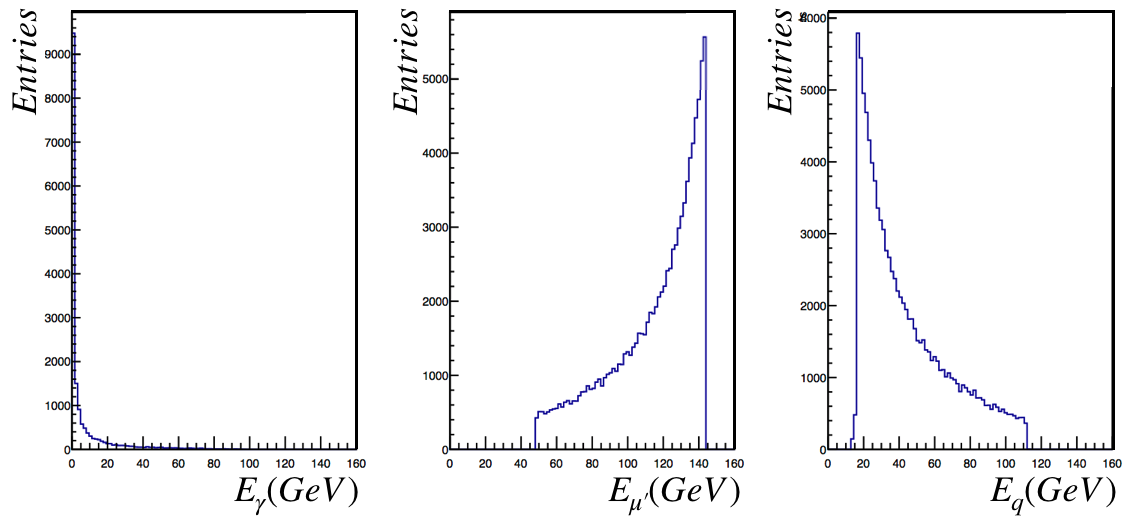
\epsfig{file=gfx/Edist.png,width=17cm}}
\caption{Energy distribution for, from left to right, radiative photon, outgoing lepton and struck quark. The emission of low energy radiative photon is privileged by DJANGOH, while the rest of the energy is distributed between the outgoing muon and the struck quark.} \label{fig:edist}
\end{figure}

We expect naively a peak around $E_{\gamma} = 0$ as soft photons (low energy photons) are more likely to be emitted than hard photons (high energy photons). The rest of the energy of the incoming muon is distributing accordingly between outgoing muon and struck quark.

Fig.~\ref{fig:anglesp} shows the $\theta_{\gamma}$ and $\theta_{\mu}$
distributions. As discussed before in Chapter~\ref{ch:Renorm}, the radiated photon has two privileged directions of emission, namely the s-peak and the p-peak, collinear to the direction of propagation of the incoming and outgoing muons. In Fig.~\ref{fig:anglesp}, the two distributions are plotted next to each other, enabling to see if the p-peak is matching with the position of the peak in the scattering angle of the outgoing muon, which is the case. The s-peak is around $0$, which is also expected.

A last exercise that I have done is to see whether DJANGOH, when we put a $Q^2>1$ constraint on event generation, is producing radiative events with $Q^2<1$, which would be the case if a radiative photon was emitted by the incoming lepton. A quick proof of this can be made starting from the relation between $Q^2_{lep}$ and $Q^2_{had}$ :

\[Q^2_{had}=Q^2_{lep}+2E_\gamma(\nu_{lep}-\sqrt{\nu_{lep}^2+Q^2_{lep}}cos\theta_\gamma)\]

When a real photon is emitted by the incoming lepton, $cos\theta_\gamma \simeq 1$ then $\nu_{lep}-\sqrt{\nu_{lep}^2+Q^2_{lep}}$
$cos\theta_\gamma \leq 0$ leading to $Q^2_{had} \leq Q^2_{lep}$. With an analoguous reasoning, if a real photon is emitted by the outgoing lepton, then $Q^2_{had} \geq Q^2_{lep}$. In Fig. \ref{fig:Q2corr}, $Q^2_{had}$ is shown as a function of $Q^2_{lep}$, for $Q^2_{lep}=1$. Values of $Q^2_{had}$ can be found both above and below $Q^2=1$, which was the point to be verified. Another information that is given by this plot is that as the distribution around $Q^2_{had} = Q^2_{lep}$ is narrow, most radiative photons are soft, ie. low energetic, as noted previously.

\begin{figure}[htb]
\centerline{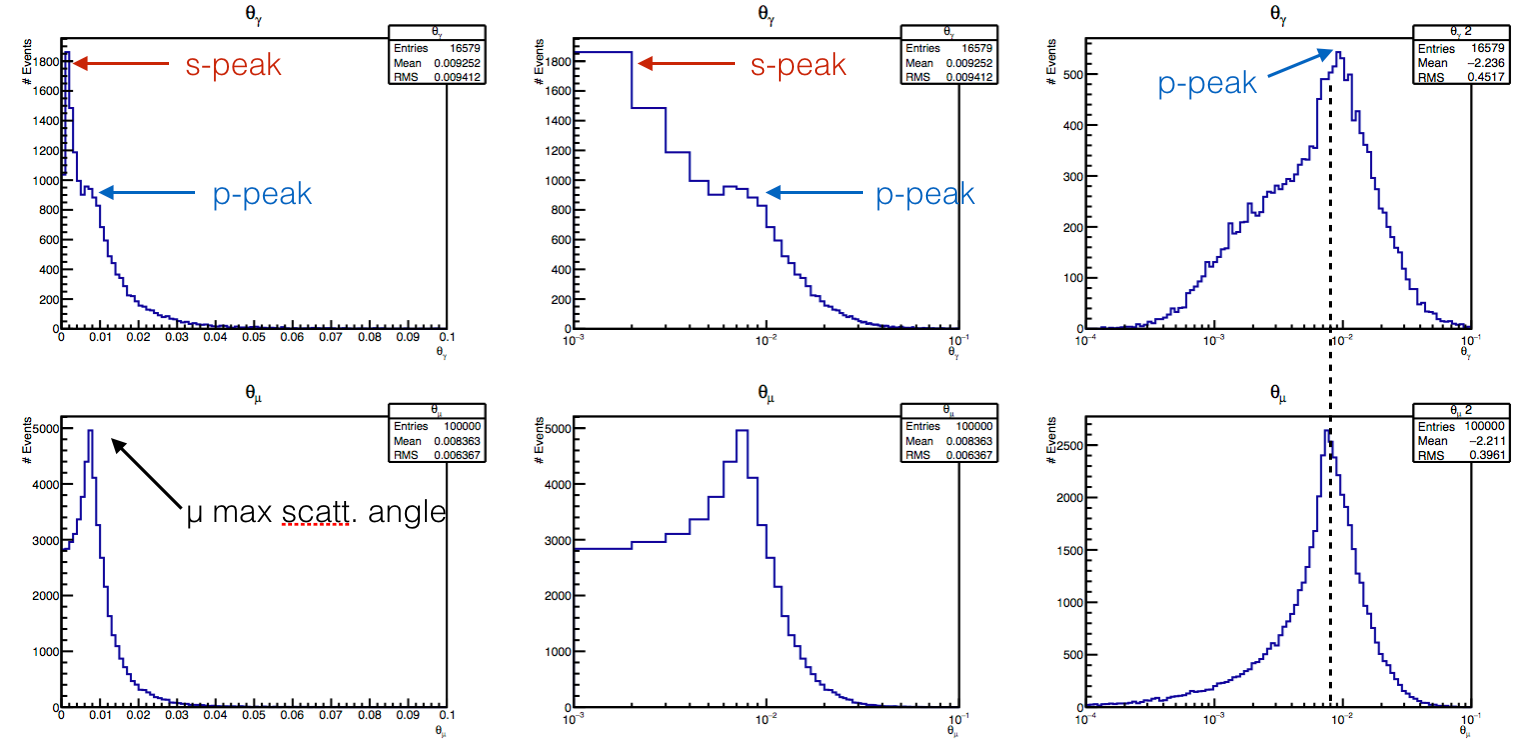
\epsfig{file=gfx/anglesp.png,width=16cm}}
\caption{$\theta$ angle distribution for the radiative photon (up) and the outgoing muon (down). From left to right the scaling of the x-axis is changed (normal, logarithmic, logarithmic with constant bin size). One can see two peaks in the theta distribution of the radiative photon : one around zero (s-peak) and one a little bit further (p-peak). When compared to the $\theta$ distribution of the outgoing muon, especially with the last scaling, one can see the two peaks match.}\label{fig:anglesp}
 \end{figure}
\hfill
\begin{figure}[htb]
\centerline{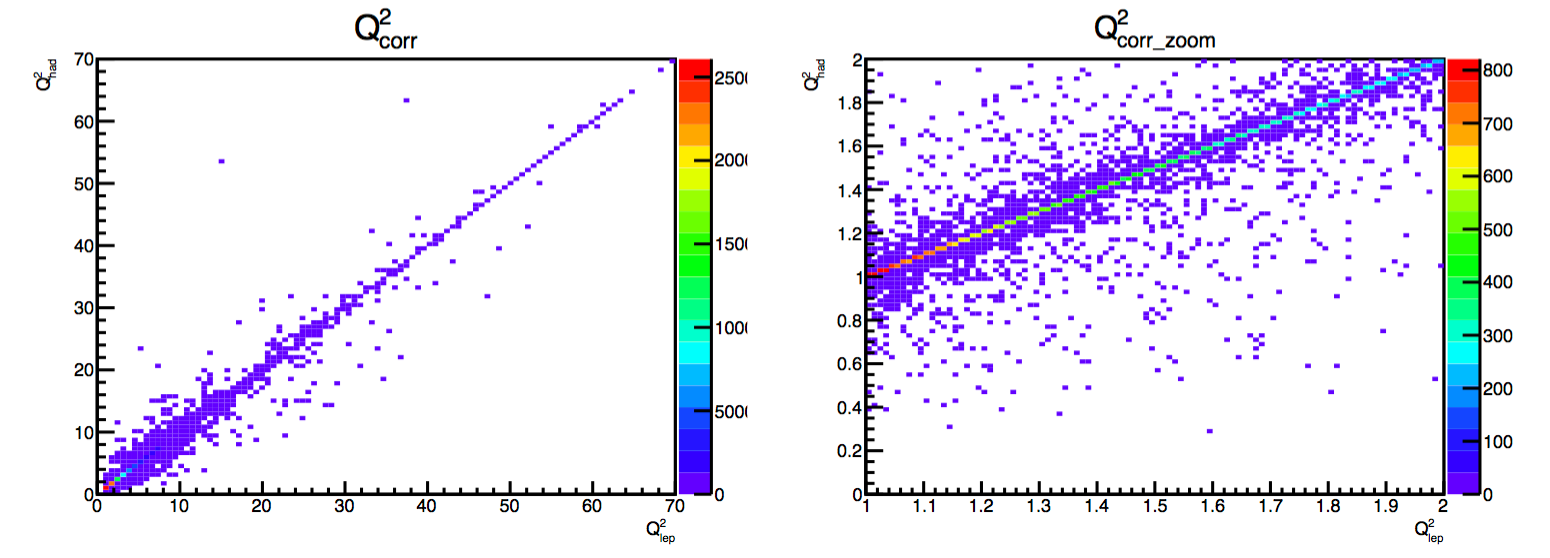
\epsfig{file=gfx/Q2_corr.png,width=16cm}}
\caption{$Q^2$ correlation plot $Q^2_{had}=f(Q^2_{lep})$. On the left is the plot for the complete range of $Q^2$
given by the kinematic constraints. The scattering around the $Q^2_{had} = Q^2_{lep}$ line is small, indicating that
most of the radiative photons are soft. On the right is the same plot but restricted to the $Q^2_{lep}\in[1,2]$ and
$Q^2_{had}\in[0,2]$ region. The fact is that for $Q^2_{lep}=1$, $Q^2_{had}$ takes values above and below $Q^2=1$, as expected.}\label{fig:Q2corr}
\end{figure}

\subsection{Enhancement of DJANGOH}

An upgrade to the original DJANGOH is the possibility to use different input energies for the incoming lepton for mutiple event generation. It was before only allowed to specify one input energy at the launch of the program. DJANGOH is now capable to take into account a new beam energy at each new event. Nonetheless, using different input energies for event generation is causing a problem : the cross-sections that are needed for event generation are depending on this input energy. The naive way would be to recompute the cross-section for each event but this solution takes much time due to the computation of the cross-section being the slowest part of the generation.

\begin{figure}[htb]
\centerline{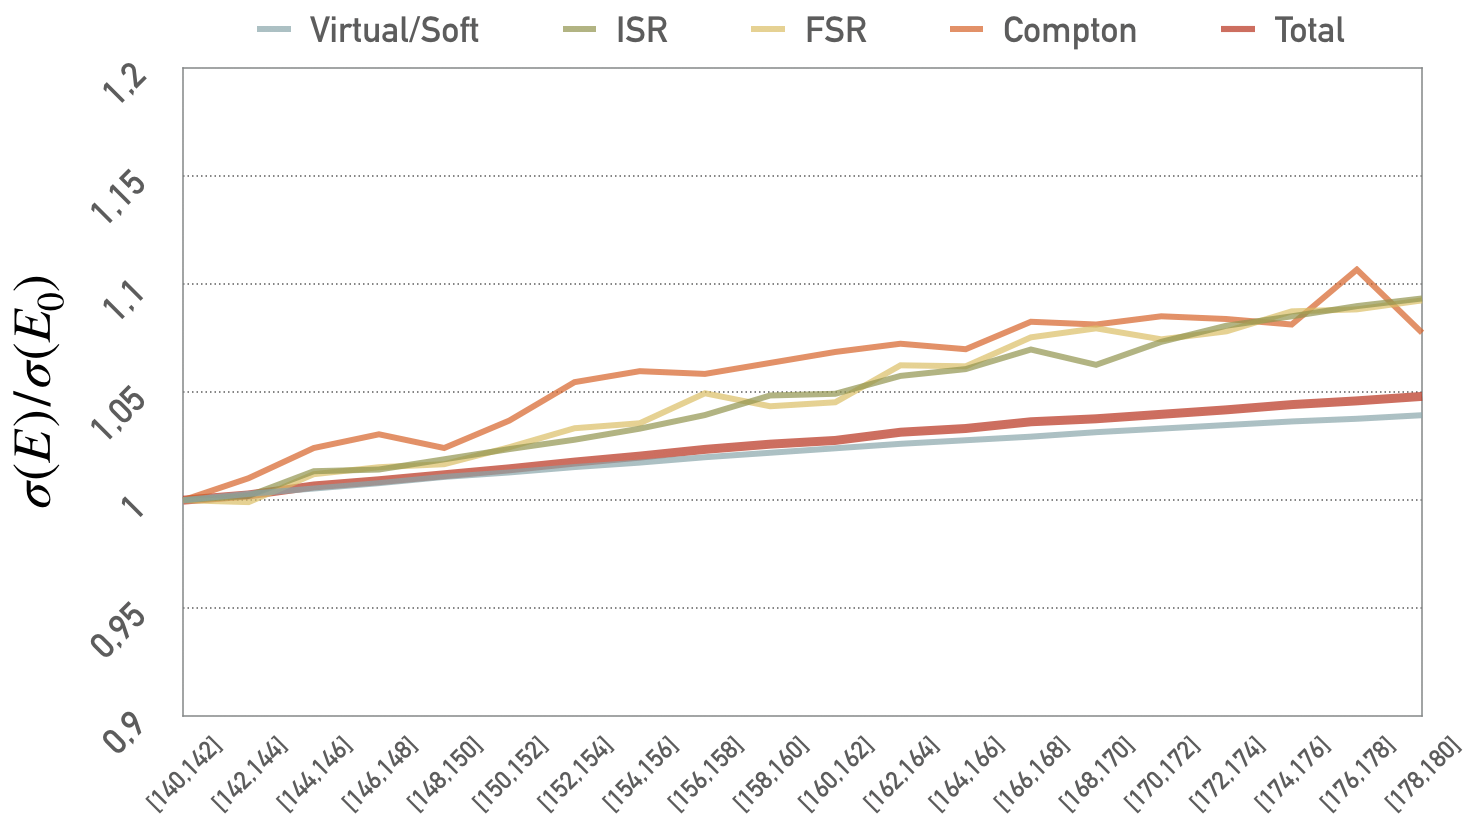
\epsfig{file=gfx/gridxs.png,width=16cm}}
\caption{Ratios of cross-section in a given energy bin over the cross-section value at $140$ GeV for virtual/soft cross-section (gray blue), initial state radiation cross-section (green), final state radiation cross-section (yellow), compton contribution cross-section (orange) and the total cross-section (red). The variation of the total cross-section with the energy goes up to $5$\%.}\label{fig:gridxs}
\end{figure}

A solution to circumvent this problem is the use of a grid of cross-sections. This grid is initialized after a rough specification of the type of dispersion in energy of the considered beam. Basically, the grid needs to have a mean energy and the standard deviation of energy to this mean energy, as well as the number of bins in the grid. Then for each bin, the energy of the center of the bin is taken and the cross-section corresponding to this energy is computed. The narrower the bins are the more accurate the cross-section is for the considered bin. As shown in Fig.~\ref{fig:gridxs}, with a mean energy of $160$ GeV, a distribution width of $20$ GeV and $20$ bins, the grid is giving an accurate map of the cross-sections. Though the difference of cross-section is not very large ($5$\% of the total cross-section), it has to be taken into account for a proper event generation.

\subsection{TDJANGOH Interface}

In order to create a C++ class (called TDJANGOH) that plays the role of an interface, I had to modify some FORTRAN parts of DJANGOH, especially the input method. DJANGOH is working with an input file where codewords with set values are specified in order to configure the generator. This was not convenient for the idea of an interface. Thus I have drawn correspondences between Common Blocks in FORTRAN and structures in C++ so that I can specify values in the C++ structure and the change is repercuted in the FORTRAN code and vice-versa. It is useful to specify the values for the input but also to recover the results of the hadronization that are located in the LUJETS Common Block. The idea is that within TGEANT the user specifies the input for DJANGOH, the interface pass it to the generator and the interface recovers the results of the generator and pass it to TGEANT (see Chapter~\ref{ch:MC}).

%----------------------------------------------------------------------------------------

\section{Summary}

The DJANGOH event generator including radiative events has been modified to simulate $\mu p$ interactions at the COMPASS experiment. After this modification, several consistency checks were performed. All were conclusive. Some further improvements were brought to the generator. The generator was designed to only work with one input energy and now can work with multiple input energies thanks to a system of cross-section grid binned in beam energy. DJANGOH being a FORTRAN framework at the age of C++, a C++ shell was built as an C++ interface to DJANGOH named TDJANGOH.
